% This is samplepaper.tex, a sample chapter demonstrating the
% LLNCS macro package for Springer Computer Science proceedings;
% Version 2.21 of 2022/01/12
%
\documentclass[runningheads]{llncs}
%
\usepackage[T1]{fontenc}
% T1 fonts will be used to generate the final print and online PDFs,
% so please use T1 fonts in your manuscript whenever possible.
% Other font encondings may result in incorrect characters.
%
\usepackage{graphicx}
\usepackage{amsmath}
\usepackage{booktabs,multicol,multirow,tabularx,array}          % Packages para tabela
\usepackage{makecell}
% Used for displaying a sample figure. If possible, figure files should
% be included in EPS format.
%
% If you use the hyperref package, please uncomment the following two lines
% to display URLs in blue roman font according to Springer's eBook style:
%\usepackage{color}
%\renewcommand\UrlFont{\color{blue}\rmfamily}
%\urlstyle{rm}
%
\begin{document}
%
\title{Human-Computer Interaction approach with Empathic Conversational Agent and Computer Vision}
%
\titlerunning{HCI approach with Empathic Conversational Agent and Computer Vision}
% If the paper title is too long for the running head, you can set
% an abbreviated paper title here
%
\author{Rafael Pereira\inst{1}\orcidID{0000-0001-8313-7253} \and
Carla Mendes\inst{1}\orcidID{0000-0001-7138-7124} \and
José Ribeiro\inst{1}\orcidID{0000-0003-3019-1330} \and
Nuno Rodrigues\inst{1}\orcidID{0000-0001-9536-1017} \and
António Pereira\inst{1,2}\orcidID{0000-0001-5062-1241}}
%
\authorrunning{Pereira, R et al.}
% First names are abbreviated in the running head.
% If there are more than two authors, 'et al.' is used.
%
\institute{Computer Science and Communications Research Centre, School of Technology and Management, Polytechnic of Leiria, 2411-901 Leiria, Portugal \\ \email{\{rafael.m.pereira, carla.c.mendes, jose.ribeiro, nunorod, apereira\}@ipleiria.pt} \and
INOV INESC Inovação, Institute of New Technologies, Leiria Office, 2411-901 Leiria, Portugal\\}

%
\maketitle              % typeset the header of the contribution
%
\begin{abstract}
The abstract should briefly summarize the contents of the paper in
150--250 words.

\keywords{First keyword  \and Second keyword \and Another keyword.}
\end{abstract}
%
%
%

\section{Introduction}

Empathy, which entails comprehending and sharing others' emotions to forge emotional connections, is vital for human relationships. Similarly, in Human-Computer Interaction (HCI), empathy is crucial in ensuring more realistic, improved, convenient and meaningful interactions. However, the typical HCI, aimed at tailoring computer systems to meet the specific needs and preferences of individuals, still lacks the users' emotional state, therefore losing crucial information during these interactions \cite{jaiswal_facial_2020}.  Recent Artificial Intelligence (AI) techniques, such as Emotion Recognition (ER) and empathic conversational agents, when integrated with HCI allow for continuous understanding of the user's emotions throughout interactions and empathically providing responses, greatly contribute to an increase in the quality and deepness of interactions between humans and computers, improving the user's overall experience \cite{santos_approaches_2018}.

Artificial Intelligence (AI) encompasses various techniques and methodologies aimed at enabling machines to perform tasks that typically require human intelligence, whereas Deep Learning (DL) stands out as a specialized approach relying on Artificial Neural Networks (ANNs) to process unstructured data (including images, voice, videos, and text, among others). ER, being a recent application of AI combined with DL, involves detecting human emotions through various modalities ranging from facial features, gestures, and poses, to speech and text captured through continuous interactions with the user \cite{alrowais_modified_2023}.  conversational agents consist of computer programs designed to simulate human-like conversation and engage in interactions with users through natural language using various techniques, including natural language processing (NLP), ML, and DL, to understand user input, interpret context, and generate appropriate responses.
 
Due to the immense potential of ER and conversational agent, individually, and the numerous benefits provided when integrated with HCI, this study offers a comprehensive guide covering ER modalities and key design and functionality aspects of a conversational agent, furthermore reviewing widely adopted datasets and methodologies. Lastly, proposing an innovative HCI approach to ensure more realistic and meaningful interactions by leveraging HCI in conjunction with ER techniques and an empathic conversational agent.
 
The primary findings of this study can be summarized as follows:
\begin{itemize}
	\item Detailed guide on how DL impacts HCI nowadays;
	\item Performed a literature review regarding ER and conversational agents;
	\item Explored the main methods and datasets used for ER and conversational agents;
	\item Proposal of a taxonomy encompassing HCI, DL, conversational agent, and ER;
	\item Proposal of an architecture of an HCI approach aided with ER, through Computer Vision (CV) and Sentiment Analysis (SA), and emphatic conversational agent.
\end{itemize}

This research is organized into six sections. Section \ref{sec:background} presents the main concepts behind DL, ER, and conversational agent. Section \ref{sec:datasets} details the most used datasets to train, validate, and evaluate ER and conversational agent algorithms. Section \ref{sec:methods} introduces and discusses the core AI algorithms used nowadays to build ER systems and conversational agents, while Section \ref{sec:solution} presents the architecture, features, and characteristics of our proposed solution for HCI aided with ER and an empathic conversational agent. Lastly, Section \ref{sec:conclusions}  introduces the challenges and directions for future work and the conclusions. 

\section{Background}
\label{sec:background}

The evolution of technology has led to an increased demand for advanced HCI. These include voice recognition, face recognition, and gesture recognition, which are essential for facilitating more natural and intuitive interactions between humans and computers \cite{Alrowais2023}. Furthermore, the ability of machines to perceive and interact with humans, whether in physical or virtual environments, needs an understanding of human motion \cite{Martinez2017}.

DL, a subset of Machine Learning (ML), has been crucial in advancing the capabilities of HCI. This has significantly enhanced performance in domains like speech recognition, visual object recognition, object detection, and even fields like drug discovery and genomics. The focus of this paper will be on supervised learning, a predominant form of DL. Supervised Learning (SL) involves training a system with a labeled dataset, where the system learns to map inputs to outputs based on example input-output pairs. During training, the system iteratively adjusts its parameters to minimize the difference between its outputs and the desired outputs \cite{Lecun2015}~\cite{Mahony2020}.

The DL processes rely on gathering and processing data for image-based models. The quality of data is crucial for a model's learning efficacy. To mitigate issues such as overfitting, which refers to the phenomenon where a network learns a function with very high variance to perfectly model the training data \cite{Shorten2019}, data augmentation can be used. This technique generates new training samples by applying transformations like rotation and scaling. It's essential for diversifying the training dataset, particularly in cases of low amounts of data \cite{Khalifa2022}.

The shift from hand-engineered features to trainable multilayer networks, namely Convolutional Neural Networks (CNNs), is a concept realized through the implementation of backpropagation. This method allows the calculation of gradients in multilayer structures by working backward from the output. CNN architecture, shown in Figure \ref{fig:cnnarchitecture}, is structured with convolutional and pooling layers. These networks process multi-array data, like images, using local connections and shared weights. The convolutional layers consist of units organized in feature maps connected to local patches in previous layers, highlighting the principle of location invariance in data like images that fit when detecting emotions through computer vision \cite{Lecun2015}.

\begin{figure}[htb]
\centering
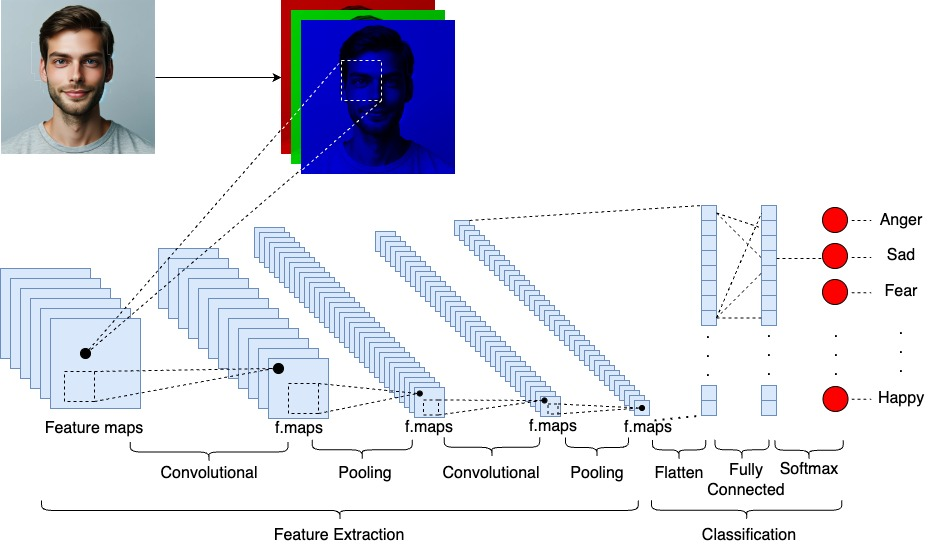
\includegraphics[width=0.97\linewidth]{CNNArchitecture.jpg}
\caption{An illustrative diagram of a CNN for emotion detection. The process begins with an input image of a smiling person and progresses through successive convolution and pooling layers for feature extraction. After flattening the feature maps, a fully connected network follows, leading to a final classification layer that categorizes the detected emotions into anger, sadness, fear, and happiness.}
\label{fig:cnnarchitecture}
\end{figure}

In CNN architecture, convolutional layers extract key features through their feature maps, while pooling layers further refine them by reducing their spatial size. This process improves the computational efficiency, and also increases the robustness of the features, a relevant aspect in the context of CV. Following this, the flattened layer transforms the two-dimensional feature maps into a one-dimensional vector, preparing them for the classification stage. This stage primarily involves fully connected layers, which interpret the extracted features and make decisions. The last layer typically employs a softmax function, shown in equation \ref{eq:sofmax}, converting the output into probabilities for each class. In this context, TL emerges as a significant strategy, allowing the transfer of knowledge from one model to another, particularly beneficial when training data is limited. It involves using pre-trained models on large datasets and adapting them to specific tasks, significantly reducing the need for extensive training data and computational resources \cite{Khan2020}.

\begin{equation}
\text{softmax}(z_i) = \frac{e^{z_i}}{\sum_{k=1}^{K} e^{z_k}} \quad \text{for} \, i = 1, 2, ..., K
\label{eq:sofmax}
\end{equation}

Emotion detection encompasses the analysis of various human expressions gathered through different modalities. In CV, it includes the detection of macro-expressions, micro-expressions, and body expressions from images and videos. These expressions provide insights into emotional states through facial movements and body language. In the non-visual domain, emotion is detected from voice, tone, and speech spectrograms, where vocal nuances reflect emotional states. Text-based emotion detection, also known as SA, on the other hand, interprets written language to identify emotions, analyzing word choice and sentence structure. Each modality presents unique challenges and requires specialized models for effective emotion recognition \cite{Chul2018}~\cite{Trigeorgis2016}~\cite{Karna2020}.

For Speech Emotion Recognition (SER), deep convolutional recurrent networks have emerged as highly effective. These networks merge the feature extraction efficiency of CNNs with the sequential data processing ability of Long Short-Term Memory (LSTM) networks. The integration of CNNs and LSTMs in these networks shows a notable advancement over traditional methods reliant on hand-engineered features \cite{Trigeorgis2016}. When detecting emotion from text, unlike other sources of expression where CNNs are used, LSTM-based models are the most used in this context. This method is effective in identifying emotional states from textual data, showcasing the ability of DL models to comprehend and process human emotions in written form \cite{Karna2020}.

Emotion recognition enables conversational agents to engage authentically by understanding and responding to users' emotions, fostering a more empathetic and natural interaction experience. A conversational agent  can be defined as a computer program that aims to interact with users realistically and naturally through simulated voice and/or textual messages, possessing either a virtual or physical body with appearances resembling humans, animals, objects, and abstract shapes, amidst others \cite{aljaroodi_avatars_2019}. Nowadays, conversational agents are applied to numerous fields with purposes ranging from entertainment, task completion, knowledge seeking, and in some instances automating previous human tasks, where they can either initiate and hold interactions in a particular domain and switch to another anytime or be bound to a single domain \cite{fernandes_survey_2020}~\cite{ramesh_survey_2017}.

The capability to deliver accurate and meaningful responses to user requests is a critical factor that greatly influences the user experience with a conversational agent. These responses can be achieved through various approaches, namely rule-based, retrieval-based, or generative-based. In the rule-based approach, the responses are static, where the model merely uses human-made rules to match the input to a pre-defined response from a limited set, therefore being the simplest to implement where the responses often lack meaningfulness and accuracy \cite{mohamad_suhaili_service_2021}. 

Similarly, a retrieval-based model queries a pre-constructed conversation repository and uses NNs to choose the response that best matches the input. This approach, although better than the first by replacing human-made rules with AI techniques, still suffers from the issue of a static conversation repository where the responses are predefined \cite{ramesh_survey_2017}. A generative-based approach uses NLP algorithms to extract the interaction's intent, entities, and context from the user's inputs while employing advanced AI techniques for text generation therefore providing consecutive unique responses, with the only downside of implementation complexity due to requiring a considerable portion of training and testing data \cite{ramesh_survey_2017}.

\section{Proposed solution}
\label{sec:solution}

% Introduction of the proposed  solution:
% 	[X] - Briefly restate the problem your solution aims to solve.
% 	[-] - Introduce your multi-modal deep learning approach, emphasizing its novelty and potential benefits.
% It's missing we emphasise the novelty and the potential benefits
Empathy is a fundamental trait in ensuring realistic, natural, and meaningful interactions in the field of HCI, therefore this section will delve into the proposed HCI approach architecture consisting of six modules as detailed in Figure \ref{fig:approachArchitecture}. Early emotion recognition mainly focused on text or facial features alone, however, humans express emotions in a highly complex way, depending on both verbal and non-verbal cues like facial expression, behavior, voice, text, and physiological signals \cite{ezzameli_emotion_2023}~\cite{zhu_multimodal_2023}. Therefore, this article proposes an architecture, for mobile devices, to diminish this issue, composed of a conversational agent module, to interact continuously with the user, and a multimodal emotion recognition module, where multiple modalities (text, audio, and video) are analyzed simultaneously with DL algorithms to better recognize human emotions and gathered together to a final emotion using a fusion model which capitalizes on the strengths of each modality and compensates for potential limitations in individual modalities. Therefore, an implementation of our proposed architecture can lead to a more engaging, empathic, and natural conversational experience with a more robust and accurate emotion recognition while being suitable for applications where natural communication involves text, speech, or visual cues simultaneously.

% CA module
Upon the capture of interaction with the user, the textual input obtained from a chat section (although if obtained as speech from the microphone it must be first converted to text using automatic speech recognition (ASR) algorithm aided with the speech spectrogram) is passed on to the NLP stage, where the input goes to some pre-processing stages such as segmentation, tokenization, lemmatization, and PoS tagging. Then, the processed data is passed through the Natural Language Understanding (NLU) stage, to extract the intents and entities while turning the pre-processed data into a structured representation. Afterward, the data is passed on to the Dialogue Management stage, which aims to maintain and incorporate the context of the current and past conversations \cite{rizou_multilingual_2022}. Finally, by analyzing the contextual data, the structured representation of the user's input, and the emotion obtained from the fusion model, the Large Language Model (LLM) provides an accurate response which is converted into a user-readable format and presented back to the user.


% SA & SER
As previously detailed, the system could gather the speech or textual data resulting from ongoing, real-time, interactions with the conversational agent, complementing this, visual data could be obtained from the camera embedded in the mobile device, either in real-time or in video, capturing facial and body pose information. Hence, the multimodal ER module analyzes in parallel all the present modalities, starting with textual data being analyzed by an SA model to obtain the sentiment conveyed in the textual input, following preprocessing, feature extraction, and classification steps. Nowadays, SA is shifting from the early key-word comparisons approach to the adoption of ML (Support Vector Machines (SVM), Naive Bayes, Maximum Entropy), DL algorithms (CNN, ensemble of CNNs) and NNs (LSTM, DNNs), and even hybrid approaches \cite{hung_beyond_2023}.



On the other hand, the speech input can be transcribed and analyzed with ASR algorithms, including deep learning techniques such as Hidden Markov Models (HMMs), Support Vector Machines (SVM), various types of Artificial Neural Networks (ANNs) such as Radial basis functions (RBF), Recurrent Neural Networks (RNNs), and Convolutional Neural Networks (CNNs), employed to extract para-linguistic information, such as intonation, duration, prosody, pitch, and rhythm, from the speech signal \cite{malik_automatic_2021}.

On the other hand, the video input data, obtained from the CV algorithm that would capture,  also continuously and in real time, the user's macro-facial expressions and body pose are passed on to a FER network and BER to further extract the emotional data conveyed in both input types.

The final stage to obtain a congregated emotion implies the usage of fusion models e.g. a late fusion model (also known as decision-level fusion) where firstly the emotion predictions are obtained from each network, and then the results based on these predictions are integrated into the final result through different decision-making methods e.g. average, majority, weighted, or other statistical strategies, this approach is usually lightweight, flexible, and versatile to change in modalities \cite{zhu_multimodal_2023}.

% Overview of the Multi-modal System:
% 	[-] - Describe the overall architecture of your system.
% 		Here we could address where the data could be gathered from (several possibilities).
% 	[-] - Explain how it integrates different modalities (speech spectrogram, transcribed text, facial and body information) for emotion detection.
%		It would be nice to emphasise deeply that we want to gather the spectrogram from the speech, that we are detecting Macro-Facial Emotions.


% Detailed Description of Each Module (Suggested methods, using kinda a Related Work of the topic it self):
% 	[] - Speech Spectrogram Analysis:
%		[] - Explain how you will process and analyze speech spectrograms for emotion detection.
%		[] - Discuss the type of deep learning models suitable for this task.
% 	[] - Sentiment Analysis Analysis:
%		[] - Describe the process of speech-to-text transcription.
%		[] - Elaborate on the techniques (like NLP algorithms) to analyze the transcribed text for emotional cues.
% 	[] - Facial and Body Information Analysis:
%		[] - Detail the methods for extracting facial and body features from video data.
%		[] - Explain the types of computer vision and deep learning techniques used for emotion recognition from these features.

% Fusion Network for Emotion Detection:
% 	[] - Describe how the outputs from the individual modules will be integrated.
% 	[] - Discuss the design of the fusion network, including how it manages and weighs inputs from different sources.
% 	[] - Explain the rationale for the chosen fusion method (e.g., weighted averaging, feature concatenation, decision-level fusion).

% Potential Challenges and Solutions:
% 	[] - Acknowledge potential challenges in implementing your proposed solution (e.g., data synchronization, dealing with ambiguous or conflicting signals from different modalities).
% 	[] - Suggest possible solutions or mitigations for these challenges.

% Expected Outcomes and Benefits:
% 	[] - Highlight what you expect the system to achieve in terms of accuracy and efficiency in emotion detection.
% 	[] - Discuss the potential applications and benefits of your approach in various domains (like HCI, psychology, user experience research).

% todo - temporary until final diagram arrives :)
\begin{figure}[htb]
	\centering
	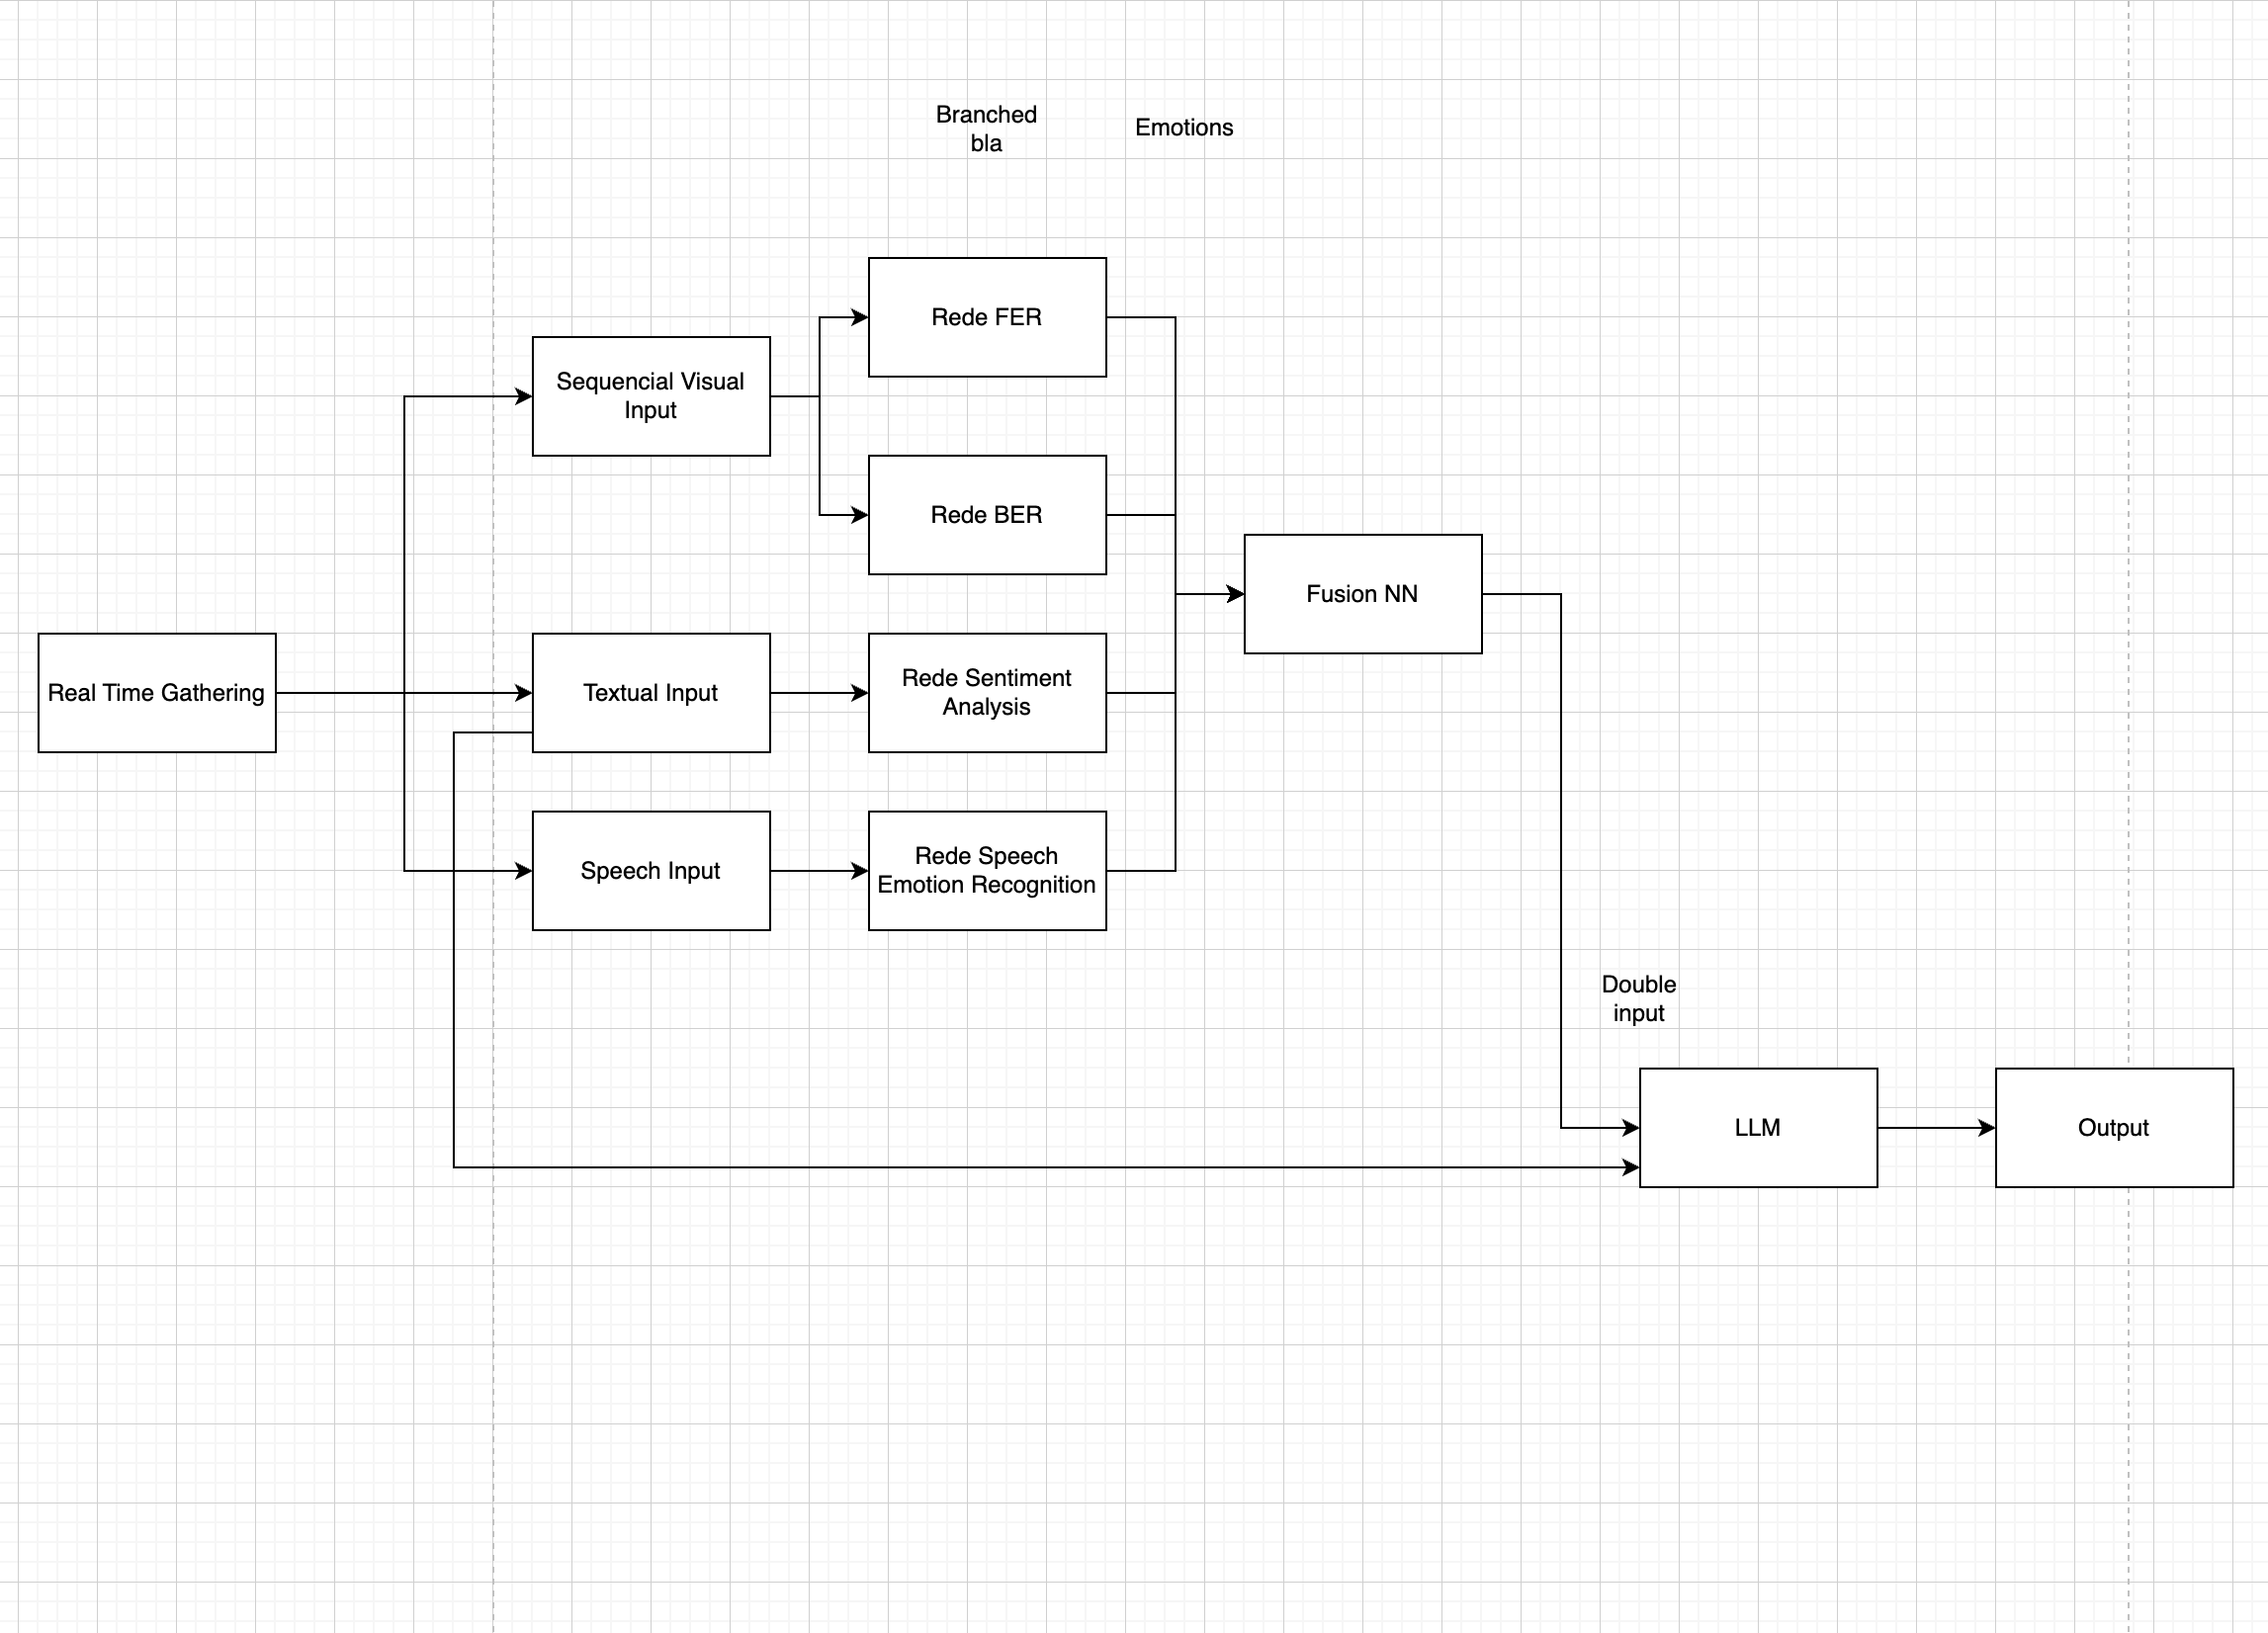
\includegraphics[width=0.97\linewidth]{approachArchitecture.png}
	\caption{HCI approach modules.}
	\label{fig:approachArchitecture}
\end{figure}

% description of characteristics
% prototype ???

\section{Future work and conclusions}
\label{sec:conclusions}

\begin{credits}
\subsubsection{\ackname} This work was supported by national funds through the Portuguese Foundation for Science and Technology (FCT), I.P., under the project UIDB/04524/2020 and was partially supported by Portuguese National funds through FITEC-Programa Interface with reference CIT “INOV-INESC Inovação-Financiamento Base”

\subsubsection{\discintname}
The authors have no competing interests.
\end{credits}
%
% ---- Bibliography ----
%
% BibTeX users should specify bibliography style 'splncs04'.
% References will then be sorted and formatted in the correct style.
%
\bibliographystyle{splncs04}
\bibliography{bibliography}
%
\end{document}
